% TODO: add in a version and date info
% TODO: operation section, led status codes
% TODO: Programmer Info copy this from the regulator datasheet and ftdi datasheet about current sourcing, drive strength electrical specs mechanical specs on the programming connector 0.1" spacing, mating connector, etc} supported baud rates
% TODO: also include recommended land pattern for programmer header (smd and through hole) also reference recommended programming cable
% TODO: add in pdf schematic

\documentclass[10pt,letterpaper]{datasheet}

\usepackage{amssymb}
\usepackage{color}
\usepackage{graphicx}
\usepackage{subfig}
\usepackage{lipsum}
\usepackage{multicol}
% \usepackage[small]{subfigure}
\usepackage{tabularx}
\usepackage[hang]{footmisc}
\usepackage{amsmath}

\newlength\SUBSIZE
\newcommand{\fixme}{{\color{red}{---FIXME---}}}
\newcommand{\mbp}{MSP430~BSL~Programmer}
\newcommand{\PIDNOLINK}{FCD\nobreakdash-PRG01}
\newcommand{\PID}{\href{http://www.flyingcampdesign.com/msp430-bsl-programmer.html}{\PIDNOLINK}}
\newcommand{\PIDURL}{\href{http://www.flyingcampdesign.com/msp430-bsl-programmer.html}{http://www.flyingcampdesign.com/msp430-bsl-programmer.html}}
\newcommand{\PIDCBLNOLINK}{FCD-CBL01}
\newcommand{\PIDCBL}{\href{http://www.flyingcampdesign.com/msp430-bsl-programmer.html}{\PIDCBLNOLINK}}
\newcommand{\PIDCBLURL}{\href{http://www.flyingcampdesign.com/msp430-bsl-programmer.html}{http://www.flyingcampdesign.com/msp430-bsl-programmer.html}}
\newcommand{\fcd}{Flying~Camp~Design}
\newcommand{\FCD}{FLYING~CAMP~DESIGN}
\newcommand{\fcdurl}{\href{http://www.flyingcampdesign.com}{www.flyingcampdesign.com}}
\newcommand{\fcdsupportemail}{\href{mailto:support@flyingcampdesign.com}{support@flyingcampdesign.com}}
\newcommand{\fcdsupporturl}{\href{http://www.flyingcampdesign.com/support.html}{http://www.flyingcampdesign.com/support.html}}
\newcommand{\tos}{\texttt{TinyOS}}
\newcommand{\tosurl}{\href{http://tinyos.net/}{\tos}}
\newcommand{\pmt}{Python~MSP430~Tools}
\newcommand{\pmturl}{\href{https://launchpad.net/python-msp430-tools/}{\pmt}}
\newcommand{\SLAUNOLINK}{SLAU319}
\newcommand{\SLAUPDF}{\href{http://www.ti.com/lit/pdf/SLAU319}{\SLAUNOLINK}}
\newcommand{\SLAUPDFURL}{\href{http://www.ti.com/lit/pdf/SLAU319}{http://www.ti.com/lit/pdf/SLAU319}}
\newcommand{\SLAUZIP}{\href{http://www.ti.com/lit/zip/slau319}{\SLAUNOLINK}}
\newcommand{\SLAUZIPURL}{\href{http://www.ti.com/lit/zip/slau319}{http://www.ti.com/lit/zip/slau319}}
\newcommand{\githuburl}{\href{http://github.com/FlyingCampDesign}{https://github.com/FlyingCampDesign}}
\newcommand{\fcdbslutility}{\href{http://www.flyingcampdesign.com/msp430-bsl-utility.html}{http://www.flyingcampdesign.com/msp430-bsl-utility.html}}

\pagestyle{fancy}
\lfoot{\fcdurl}
\cfoot{\PIDNOLINK\ Datasheet -- Rev. D}

\usepackage[pdftex,
            colorlinks=true,
            urlcolor=blue,
            hyperfootnotes=true,
            bookmarks=true,
            bookmarksopen=false,
            pdfpagemode=None]{hyperref}
\hypersetup{pdftitle={\PID\ Datasheet},
            pdfauthor={\FCD},
            pdfkeywords={msp430,BSL,bootstrap,loader,programmer}}

\begin{document}
\title{\color{red}{\bf \mbp\newline\PIDNOLINK}}
\author{\FCD}
\date{}
\maketitle
\makefooter
\thispagestyle{fancy}

\section*{Highlights}
\begin{multicols}{2}
  \begin{itemize}
    \item Supports all MSP430 device families supported by TI example "Bootstrap Loader Hardware" in \SLAUPDF\footnote{\PID\ does not include inverting buffers as shown in the TI reference hardware.  Requires PC software to support specific MSP430 device families.  Not all MSP430 devices have been tested for hardware compatibility. See page~\pageref{tab:msp430-device-support} for device family support.}
    \item Standard 6 pin, 0.1" header interface
    \item USB bus powered
    \item 3.3V target supply output (up to 400mA)
    \item Cross platform driver support for Windows, Linux, and Mac OS
    \item Full \pmturl\ support
    \item Full \tosurl\ support
    \item Fully Open-Source hardware design%
    \footnote{Design files available at \PIDURL}
  \end{itemize}
\end{multicols}

\section*{Product Description}
\begin{multicols}{2}
  The \PID\ is a USB bootstrap loader\footnote{``MSP430 Programming Via the Bootstrap Loader (\SLAUNOLINK)'' Application Note (\SLAUPDFURL)} (BSL) programmer for the Texas Instruments MSP430 microcontroller.  For designs where low cost or small form factor prohibit the integration of custom programming logic or a large JTAG header, the \PID\ enables in-system programming by including a single 6 pin header in the target device design.

  \begin{center}
    
\includegraphics[width=3 in]{fcd-prg01-diag}
  \end{center}

  Originally designed to work with the cross platform \tosurl\ toolchain, the \PID\ provides an open source, cross platform alternative to platform dependent development tools for the MSP430 microcontroller.

  \begin{center}
    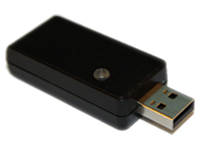
\includegraphics[width=2 in]{fcd-prg01}
  \end{center}

  The \PID\ integrates a USB-to-serial converter and on board regulated power supply into a small USB dongle, allowing programming and test capability over a single interface.  It exposes a standard 6 pin, 0.1" header which can be used to interface to the target board via a device specific cable harness.  This modular approach provides designers with the flexibility to select the optimal physical programming interface for the unique design constraints of each target platform.

\end{multicols}

\section*{Ordering Information}
\begin{flushleft}
  \label{tab:ordering}
  \begin{tabular}{l l}
    \textbf{\PID} & \mbp \\
    \textbf{\PIDCBL} & Programming interface cable (6x1, 0.1" $\leftrightarrow$ 3x2, 2mm) \\
  \end{tabular}
\end{flushleft}

\newpage

\section*{Programming Interface}
\begin{flushleft}
  The \PID\ provides a standard 6x1, 0.1" programming header for powering and communicating with the target device. \\

  \begin{figure}[!h]
    \label{fig:fcd-prg01-pinout}
    \begin{center}
      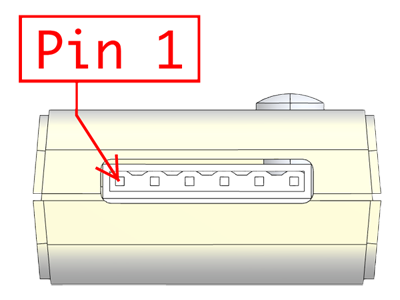
\includegraphics[width=2 in]{fcd-prg01-pinout}
    \end{center}
    \caption{6x1, 0.1" Header}
  \end{figure}

  \subsection*{Pinout}
  \begin{flushleft}
    \label{tab:pinout}
    \begin{tabular}{|c|c|c|c|}
      \hline
      \PIDNOLINK\ Signal &
      \PIDNOLINK\  Pin &
      MSP430 devices with TEST pin &
      MSP430 devices without TEST pin \\
      \hline
      DTR & 1 & TEST & TCK \\
      RXD & 2 & UART\_TX & UART\_TX \\
      TXD & 3 & UART\_RX & UART\_RX \\
      VCC & 4 & VDD & VDD \\
      RTS & 5 & RST & RST \\
      GND & 6 & GND & GND \\
      \hline
    \end{tabular}
  \end{flushleft}

  \bigskip

  \subsection*{Electrical Characteristics}
    \subsubsection*{VCC Target Supply Output (Pin 4)}
    \label{tab:elec-sup}
    \begin{tabular}{|l|c|c|c|c|c|}
      \hline
      Parameter &
      Minimum &
      Typical &
      Maximum &
      Units &
      Conditions \\
      \hline
      Output Voltage & - & 3.3 & - & V & \\
      Output Current & - & - & 0.4 & A & \\
      Short Circuit Current & - & 450 & - & mA & Vout = 0 V \\
      Dropout Voltage & - & 75 & 200 & mV & Iout = 400 mA \\
      Accuracy & - & 1 & - & \% & \\
      \hline
    \end{tabular}

    \subsubsection*{UART and I/O (Pins 1,2,3,5)}
    \label{tab:elec-io}
    \begin{tabular}{|l|c|c|c|c|c|}
      \hline
      Parameter &
      Minimum &
      Typical &
      Maximum &
      Units &
      Conditions \\
      \hline
      DC Input Voltage & -0.5 & - & 3.8 & V & \\
      Output Drive Strength & - & 12 & - & mA & \\
      Output Voltage High & 2.2 & 2.8 & 3.2 & V & Isource = 3 mA \\
      Output Voltage Low & 0.3 & 0.4 & 0.6 & V & Isink = 8 mA \\
      Input Switching Threshold & 1.0 & 1.2 & 1.5 & V & \\
      Input Switching Hysteresis & 20 & 25 & 30 & mV & \\
      \hline
    \end{tabular}
\end{flushleft}

\newpage

\section*{Programming Cables}
\subsection*{\PIDCBL}
\begin{flushleft}
  A programming cable harness which mates with standard 3x2, 2mm PCB headers is available from \fcd\ for use with the \PID.  Pinout for this cable is available in schematic form at \PIDCBL.

  \begin{figure}[!h]
    \label{fig:fcd-cbl01}
    \begin{center}
      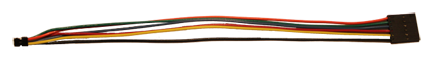
\includegraphics[]{fcd-cbl01}
    \end{center}
    \caption{\FCD\ \PIDCBLNOLINK}
  \end{figure}

  \fcd\ recommends using the following through hole and surface mount headers for use with the \PIDCBL:

  \begin{figure}[!h]
    \label{fig:rec-prog-hdr}
    \begin{center}
      \subfloat[\href{http://www.hirose.co.jp/cataloge_hp/e54305002.pdf}%
                     {Hirose DF11-6DP-2DSA(01)}]{
        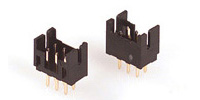
\includegraphics[width=2 in]{DF11-6DP-2DSA(01)_sml}}
      \subfloat[\href{http://www.hirose.co.jp/cataloge_hp/e54305002.pdf}%
                     {Hirose DF11G-6DP-2V(50)}]{
        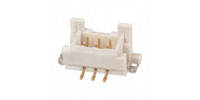
\includegraphics[width=2 in]{DF11G-6DP-2V(50)_sml}}
      \caption{Recommended headers for use with the \PIDCBLNOLINK\ cable}
    \end{center}
  \end{figure}

  A Cadsoft Eagle CAD library which contains land pattern footprints for these headers is available for download on the \PID\ product page: \PIDURL \newline

\subsection*{Custom Programming Cables}
  For those customers wishing to design their own custom programming cables, \fcd\ recommends the following mating connector for use with the 6 pin BSL programming interface:

  \begin{figure}[!h]
    \label{fig:50-57-9006}
    \begin{center}
      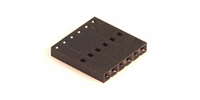
\includegraphics[width=2 in]{50-57-9006_sml}
    \end{center}
    \caption{\href{http://www.molex.com/pdm_docs/sd/050579006_sd.pdf}%
                  {Molex 50-57-9006}}
  \end{figure}

\end{flushleft}

\newpage

\section*{Installation}
\begin{flushleft}
  The \PID\ uses a USB $\leftrightarrow$ Serial interface chip (\href{http://ftdichip.com/Products/FT232R.htm}{FTDI Chip FT232R}) and corresponding operating system driver to provide a Virtual COM Port (VCP) interface layer to the BSL programming software.  The BSL programming software depends upon this VCP interface layer to control the communication pins on the programmer.\\
  \begin{enumerate}
    \item \textbf{Before plugging in the \PID\ to your computer}, install the appropriate driver for your operating system by following the corresponding installation guide available online at: \newline
    \href{http://ftdichip.com/Documents/InstallGuides.htm}{http://ftdichip.com/Documents/InstallGuides.htm} \newline

    A full listing of the latest VCP drivers for all supported operating systems is available online at: \newline \href{http://ftdichip.com/Drivers/VCP.htm}{http://ftdichip.com/Drivers/VCP.htm} \newline

    \textbf{Note:} A Linux driver for the FT232R is included in most newer kernels ( $>$ 2.4.20 or greater).  However, on some kernels an older F232BM driver may be used which is compatible with the FT232R.  \newline

    \item After installing the appropriate driver for your operating system, insert the \PID\ into a free USB port on your computer.

    \item If installation was successful, the \PID\ should appear as a VCP on your computer:

    \label{tab:elec-io}
    \begin{tabular}{l l}
      \textbf{Windows} & COM[X] \\
      \textbf{Linux} & /dev/ttyUSB[X] \\
      \textbf{Mac OS X} & /dev/tty.usbserial-[...] \\
    \end{tabular}
  \end{enumerate}
\end{flushleft}

\newpage

\section*{MSP430 Device Family Support}
\begin{flushleft}
    Any MSP430 device family that is supported by the example hardware described in \SLAUPDF\ section 4.1 "Hardware Description" should also be compatible with the \PID.  The following table provides information about MSP430 device families that are not compatible with the \PID\ hardware.
\end{flushleft}
\label{tab:msp430-device-support}
\begin{tabularx}{\textwidth}{|c|X|}
  \hline
  Device Family &
  Summary \\
  \hline
  MSP430F543xA & \PID\ is incompatible with MSP430F543xA family devices.  There is a bug in the MSP430F543xA family which requires that the second low pulse on TEST must be shorter than 15us, which the VCP drivers for the \PID\ are unable to achieve. Please reference SYS10 in \href{http://www.ti.com/litv/pdf/slaz290b}{http://www.ti.com/litv/pdf/slaz290b} for more details.\\
  \hline
\end{tabularx}

\newpage

\section*{Software Support}
\begin{flushleft}
The Virtual COM Port (VCP) drivers provide a serial port interface to the BSL control software.  This generic software interface enables the use of third party BSL tools, as well as provides a simple abstraction to those users wishing to write their own BSL tools.  The mapping between the VCP signal and the programmer pins is shown in the table on page~\pageref{tab:pinout}.  The following examples show how to use the \PID\ with the BSL tools available from TI and a couple popular MSP430 toolchains.

\subsection*{TinyOS}
The \tos\ toolchain includes built in support for the \PID.  The following example can be used to compile a \tos\ application and install it onto an MSP430 based \tos\ ``platform'':
\begin{verbatim}
    make [platform] install miniprog
\end{verbatim}
More information about the \tos\ toolchain is available online at: \tosurl
\end{flushleft}

\subsection*{\SLAUNOLINK}
The TI support files\footnote{\SLAUZIPURL} for \SLAUPDF\ include a command line demo utility for communication with 1/2/4xx BSLs.  This utility is called "BSLDEMO2.exe" and is designed to work with the example hardware described in \SLAUPDF\ section 4.1 "Hardware Description".  The \PID\ mimics this hardware by providing a VCP interface to the BSL control software.  However, the \PID\ does not include inverting buffers on RST and TCK as shown in the TI reference hardware.  Furthermore, the \PIDCBL\ swaps the RST and TCK pins (with respect to the virtual COM port RTS and DTR pins).  Therefore, the BSLDEMO2.exe utility source code provided by TI must be patched and recompiled to work correctly with the \PID\ + \PIDCBL\ combination.  A patched version of BSLDEMO2.exe can be downloaded from \PIDURL\ while the source can be obtained from \githuburl.  The following example programs the target with the TI-TXT firmware file ``firmware.txt'':
\begin{verbatim}
    BSLDEMO2.exe -s2 -cCOMx firmware.txt
\end{verbatim}

\subsection*{\pmt}
The \pmturl\ project includes built in support for the \PID.
The \pmt\ can be installed from \href{http://pypi.python.org/pypi/python-msp430-tools/}{http://pypi.python.org/pypi/python-msp430-tools/} via ``pip'' by running:
\begin{verbatim}
    pip install pyserial python-msp430-tools
\end{verbatim}
The following example clears all flash memory, programs the target with the Intel HEX firmware file ``firmware.hex'', and then resets the target:
\begin{verbatim}
    msp430-bsl-fcdprog.py -p /dev/path-to-msp430-bsl-programmer -r -e path/to/firmware.hex
\end{verbatim}

\subsection*{MSP430 BSL Utility (no longer under active development)}
The \fcd\ MSP430 BSL Utility is an open source GUI utility which was designed to be fully compatible with the \PID. Open source code can be obtained from: \githuburl \newline More information about using the \PID\ with this software is available on the MSP430 BSL Utility product page: \fcdbslutility

\newpage

\section*{Questions?}
Contact \fcdsupportemail\ or visit \fcdsupporturl

\newpage

\section*{Revision History}
\label{tab:revision-history}
\begin{tabularx}{\textwidth}{|c|c|X|}
  \hline
  Revision &
  Date &
  Summary \\
  \hline
  C & 12/09/2012 & - Add MSP430 Device Support page \newline %
                   - Add Revision History page \newline %
                   - Add SLAU319 software section \newline %
                   - Update links to \pmt \newline %
                   - Add note saying MSP430 BSL Utility is no longer under active development \\
  \hline
  D & 12/11/2012 & - Add date column to Revision History table \newline %
                   - Update MSP430 BSL Utility description and add link to Github page \\
  \hline
\end{tabularx}

\newpage

\section*{Legal}

\begin{flushleft}
Flying Camp Design reserves all rights to this document and the information
contained herein.  Product names, trademarks, or logos described or
displayed herein may be subject to Flying Camp Design or third-party
intellectual property rights.  Permission to use, copy, and distribute
this document, without fee, and without written agreement, is hereby
granted, provided that the document is not modified in any manner.
\newline
\newline
In no event shall Flying Camp Design be liable to any party for direct,
indirect, special, incidental, or consequential damages arising out of
the use of this information or the hardware and software that this
document describes, even if Flying Camp Design has been advised of the
possibility of such damage.
\newline
\newline
Flying Camp Design specifically disclaims any warranties, including, but not
limited to, the implied warranties of mechantability and fitness for a
particular purpose.  The information contained herein is provided on
an ``as is'' basis, and Flying Camp Design has no obligation to provide
maintenance, support, updates, enhancements, or modifications.  This
document may be revised by Flying Camp Design at any time.
\newline
\newline
Copyright \copyright~\the\year, Flying Camp Design.  All Rights Reserved.
\end{flushleft}


\end{document}

